\documentclass[twocolumn]{article}

\usepackage{amsmath}
\usepackage{bm}
\usepackage{caption}
\usepackage{graphicx}
\usepackage{float}
\usepackage{subcaption}
\usepackage{gensymb}

% Make table names in captions boldfaced
\captionsetup[table]{labelfont=bf}
\captionsetup[figure]{labelfont=bf}

%opening
\title{Laboratory Observations of the Zeeman Effect}
\author{Jack Nelson,\footnote{With student Chongmo Tang as lab partner.}\\
	Physics Department,\\
	Occidental College, Los Angeles, CA}
\date{November 2016}

\begin{document}

\maketitle

\begin{abstract}
	We report our observations of the Zeeman effect of the 546.1 nm mercury spectral line in a 1T magnetic field.
	Using a polarizing filter, we were able to observe hyperfine structure in the spectrum from transitions with particular changes in the quantum number $M_j$, verifying through observation the properties anticipated by theory.
	We used measurements of the hyperfine structure of the ``Normal" Zeeman effect to calculate a value for the Bohr magneton, $\mu_B = 9.22\times10^{-24}\pm 0.06\times10^{-24} J\cdot T^{-1}$, which is consistent with the modern accepted value to within 0.63\% agreement.
\end{abstract}

\section{Introduction} \label{sec:Intro}
	We begin with an overview of the theory behind the Zeeman effect, then proceed into a discussion and derivation of the equation we used to calculate the value of the Bohr magneton from our measurements.
	
	\subsection{Theoretical Overview} \label{sec:Theory}
		The splitting of the spectra of mercury into hyperfine lines when an external magnetic field is applied is the result of the mercury atom's magnetic-dipole interaction with the external magnetic field.
		 
		In its ground state, the mercury atom has 80 electrons in which the n = 1, 2, 3, 4, and 5 shells are filled, leaving two 6s valence electrons.
		The spectral emissions of mercury come from the transitions of these two valence electrons between different quantum states.
		Figure \ref{fig:MercuryEnergyLevelsDiagram} shows the different possible transitions of the mercury atom.
		Our observations will be limited to the $7^3S_1 \rightarrow 6^3P_2$ transition which yields the 546.1 nm green spectral line.
		
		When no external magnetic field is present, hyperfine structure in atomic spectra can be observed due to the spin-angular momentum coupling of electrons. 
		See pp. 47 of \cite{melissinos_experiments_1966} for a more detailed discussion.
		In the presence of an external magnetic field, the interaction of the total angular momentum of the electrons with the magnetic field also splits the spectral lines into finer lines of slightly different wavelength.
		Figure \ref{fig:SpectralSplitting} shows how a single transition from the $l=2$ to $l=1$ states results in hyperfine structure in the presence of a magnetic field.
		
		\begin{figure}
			\centering
			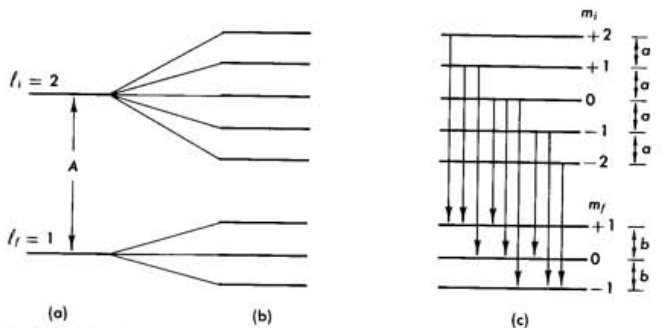
\includegraphics[width=1.0\linewidth]{Images/SpectralSplitting}
			\caption{A single spectral line caused by an atomic energy transition will be split into multiple ``hyperfine" lines due to the interaction of the total angular momentum of the valence electrons with an external magnetic field. (a) shows the transition in the absence of an external magnetic field. The transition between the $l=2$ and the $l=1$ states ($d\rightarrow p$) produces a single spectral line. (b) shows how these formerly single energy-levels are split into multiple states in the presence of an external magnetic field. (c) shows the possible transitions between the new states, each of which produces a different spectral line with slightly different wavelength.\cite{melissinos_experiments_1966}}
			\label{fig:SpectralSplitting}
		\end{figure}
		
		The following discussion is a summary of the theory behind the Zeeman effect. For more detailed discussions and derivations, see \cite{melissinos_experiments_1966} and \cite{stoltenberg_zeeman_2007}.
		
		Hyperfine splitting in the presence of a magnetic field is due to the magnetic dipole interactions of an electron with the magnetic field.
		These interactions result in an added energy $\Delta E$ per electron for a quantum state that is given by
		\begin{equation}
			\Delta E = m\mu_0B
		\end{equation}
		where $m$ is the quantum number quantifying the projection of the total angular momentum along the z-axis of the atom, $\mu_0$ is the Bohr magneton, the fundamental magnetic moment of the electron, and $B$ is the applied magnetic field.
		
		To understand the origin of these interactions, consider a simple current loop such as the one shown in Figure \ref{fig:CurrentLoopDiagram}.
		The associated magnetic moment $\mathbf{\mu}$ of the loop has the magnitude:
		\begin{equation}
			\mu = IA
		\end{equation}
		Where $A=\pi a^2$ is the disk area enclosed by the loop.
		The direction of $\mathbf{\mu}$ is given by the right-hand rule.
		
		When an external magnetic field $\mathbf{B}$ is applied, the torque on the loop is given by
		\begin{equation}
			\boldsymbol{\tau} = \boldsymbol{\mu} \times \mathbf{B}
		\end{equation}
		The resulting potential energy of the current loop in the magnetic field is
		\begin{equation} \label{eq:MagneticEnergy}
			E_{B} = -\boldsymbol{\mu}\cdot \mathbf{B}
		\end{equation}
		That is, the magnetic field will do work on the current loop when its orientation is changed in the field.
		
		Thus, we can classically model the electron as a loop of current, as shown in Figure \ref{fig:CurrentLoopDiagram}, with magnetic moment given by
		\begin{equation}
			\boldsymbol{\mu_l} = -\left(\frac{e}{2m_e}\right) \mathbf{l}
		\end{equation}
		where $m_e$ is the mass of the electron, $e$ is the electron charge, and $\mathbf{l}$ is the orbital angular momentum.
		This is then conventionally stated as
		\begin{equation} \label{eq:MagneticMoment}
			\boldsymbol{\mu_l} = -g_l \left( \frac{e\hbar}{2m_e} \right) \left(\frac{\mathbf{l}}{\hbar}\right) = -g_l\mu_B \left(\frac{\mathbf{l}}{\hbar}\right)
		\end{equation}
		where $\mu_B$ is the Bohr magneton, and $g_l$ is a unitless ``g factor" which relates the magnitude of the magnetic moment in units of $\mu_B$ to the magnitude of the orbital angular momentum in units of $\hbar$.
		This ``g factor" will be important later.
		
		\begin{figure}
			\centering
			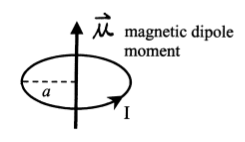
\includegraphics[width=0.7\linewidth]{Images/CurrentLoopDiagram}
			\caption{A loop of current about a vertical axis with magnetic moment $\mathbf{\mu}$.\cite{stoltenberg_zeeman_2007}}
			\label{fig:CurrentLoopDiagram}
		\end{figure}
		
		We use this classical model of the electron as a current loop to begin our theory of the Zeeman effect, but it doesn't get us far.
		For the purposes of simplicity, we will at first consider an atom with only one valence electron, such as sodium.
		Later, we will include the effect of multiple valence electrons, such as in mercury.
		\footnote{As such, we will use lower-case $lsmj$ to denote the quantum numbers of single electrons, while upper-case $LSMJ$ will be used for systems of more than one electron.}
		
		The magnetic torque on an atom is due to the coupled interaction of an electron's total angular momentum, $j$, with the magnetic field.
		The two forms of angular momentum in electrons - orbital angular momentum, $l$, and intrinsic spin momentum, $s$ - couple to form a measure of total angular momentum, $j$:
		
		\begin{equation}
		\mathbf{j} = \mathbf{l} + \mathbf{s}
		\label{eq:TotalAngularP}
		\end{equation}
		which has magnitude $\left|\mathbf{j}\right| = \sqrt{j\left(j+1\right)}\hbar$.
		Figure \ref{fig:TotalAngularMomentumDiagram} shows how these two quantities (vectors, actually) combine to form total angular momentum.
		
		The z-component of $j$, $j_z$, is also given by the sum of the z-components of $s$ and $l$
		\begin{equation}
			j_z = l_z + s_z = m_j\hbar
		\end{equation}
		where $m_j$ is the quantum number quantifying the projection of total angular momentum along the z-axis.
		
		\begin{figure}
			\centering
			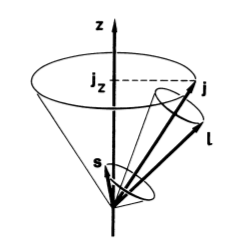
\includegraphics[width=0.7\linewidth]{Images/TotalAngularMomentumDiagram}
			\caption{Electron spin angular momentum $\mathbf{s}$ and orbital angular momentum $\mathbf{l}$ sum to create total angular momentum $\mathbf{j}$.\cite{stoltenberg_zeeman_2007}}
			\label{fig:TotalAngularMomentumDiagram}
		\end{figure}

		
		Selection rules place restrictions on how the quantum numbers may change when a valence electron undergoes a transition.
		These selection rules are:
		\begin{enumerate}
			\item $\Delta s = 0$
			\item $\Delta l = 0, \pm1$
			\item $\Delta j = 0, \pm1$, but not $\Delta j = 0 \rightarrow \Delta j = 0$
			\item $\Delta m_j = 0, \pm1$, but not $m_j=0\rightarrow m_j=0$ if $\Delta j = 0$
		\end{enumerate}
		
		From equation (\ref{eq:MagneticEnergy}), the energy change due to a magnetic field is related to the magnetic moment of the electron and the magnitude of the field.
		Using equation (\ref{eq:MagneticMoment}), we can develop an expression for the quantum-mechanically accurate energy difference of the valence electron in the presence of the magnetic field:
		\begin{equation}
			\Delta E = E_B = g_jm_j\mu_BB
			\label{eq:EnergyShift}
		\end{equation}
		
		The g factor in equation (\ref{eq:EnergyShift}) is known as the Land\'{e} g factor, and is given by
		\begin{equation}
		g_L = 1 + \frac{J(J+1) + S(S+1) - L(L+1)}{2J(J+1)}
		\label{eq:LandeGFactor}
		\end{equation}
		
		The Lande\'{e} g factor is derived from considering the projections of the spin and orbital magnetic moments along the total angular momentum j.
		\cite{stoltenberg_zeeman_2007}
		
		When we consider multiple valence electrons, under LS or Russell-Saunders coupling, we can couple together the angular momenta for more than one electron. 
		The individual orbital and spin angular momenta combine to form total angular momenta, thus $L$ and $S$ combine to form $J$ just as $l$ and $s$ combine to form $j$:
		\begin{equation}
			\mathbf{J} = \mathbf{L} + \mathbf{S}
		\end{equation}
		
		Figure \ref{fig:SpectralSplitting} shows that spectral splitting is dependent on the quantum number $m_j$.
		$m_j$ can take on $2l+1$ the values ranging from $l$ to $-l$.
		
		The polarization of the emitted light during the transition is also entirely determined by $\Delta m_j$.
		For $\Delta m_j = 0$, the emitted photons are polarized linearly and parallel to the field lines of the applied magnetic field $\mathbf{B}$.
		For $\Delta m_j=\pm1$, emitted photons are circularly polarized along the direction of $\mathbf{B}$ and appear linearly polarized perpendicular to $\mathbf{B}$ when viewed side-on to $\mathbf{B}$.
		\begin{figure}
			\centering
			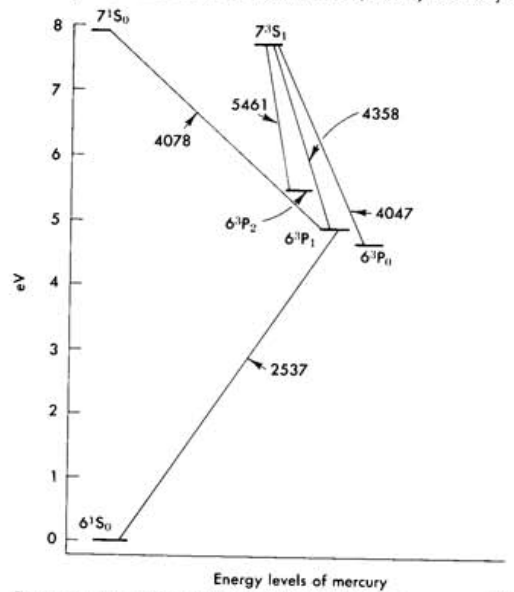
\includegraphics[width=0.5\textwidth]{Images/MercuryEnergyLevelsDiagram.png}
			\caption{Energy level transitions of mercury between quantum states. For the purposes of our observations, we are interested in the $7^3S_1 \rightarrow 6^3P_2$ transition which produces 546.1 nm light. Figure 7.39 of \cite{melissinos_experiments_1966}}
			\label{fig:MercuryEnergyLevelsDiagram}
		\end{figure}
		
		The energy difference between the hyperfine spectra is caused by the differing values of $\Delta m_j$ and determined by measuring the relative differences in wavelength between the fine spectra.
		From the basic Planck relation we have
		\begin{equation}
			E = h\nu = \frac{hc}{\lambda}
		\end{equation}
		where $h$ is the Planck constant, $\nu$ is wave frequency, and $\lambda$ is wavelength.
		
		The relative energy difference of two wavelengths is then given by
		
		
		
		\begin{equation}
			\Delta E = M_j g_L B \mu_B
			\label{eq:EnergyShift}
		\end{equation}
		
		\subsection{Calculation of the Bohr Magneton} \label{subsec:BohrCalc}
			The fundamental unit of magnetic moment, the Bohr magneton, is given by
			
			\begin{equation}
				\mu_B = \frac{eh}{4\pi m_e}
			\end{equation}
			where $m_e$ is the electron mass, $e$ is the electron charge, and $h$ is Planck's constant.
			We are interested in measuring this fundamental quantity through observation.
			To do so, we will measure the magnitude of the hyperfine spectral line splitting in the presence of a magnetic field, and relate this splitting to the magnitude of the Bohr magneton.
			
			Consider the 546.1 nm mercury line in the presence of a magnetic field.
			As described in the previous section, the interaction of the spin-coupled total angular momentum of the valence electron will interact with the magnetic field to produce hyperfine structure with energy, and thus wavelength, dependent on the value of $\Delta M_j$ in the transition.
			
			For the case of $M_j = 0 \rightarrow M_j = 0$, the resulting spectral line will be the same as the un-split spectral line in the $B=0$ case with $\lambda = 546.1 nm$.
			In the $M_j = +1 \rightarrow M_j = +1$ and $M_j = -1 \rightarrow M_j = -1$ cases, however, the resulting hyperfine spectral line will be of slightly greater or less energy than the $B=0$ spectral line, thus resulting in a ``triplet" hyperfine structure in which the central 546.1 nm spectral line is surrounded on either side by two additional hyperfine spectral lines.
			
			We calculate the Land\'{e} g-factor for both the S and P states using equation (\ref{eq:LandeGFactor}).
			For the $^3S_1$ state, $L=0$ and $S=1$, thus $J = 1$, and $g_S = 2$.
			For the $^3P_2$ state, $L=1$ and $S=1$, thus $J=2$, and $g_P = 3/2$.
			
			Thus, using equation (\ref{eq:EnergyShift}), the energy shifts for the $M_j = \pm1$ cases for the $S$ and $P$ states in the presence of a magnetic field will be:
			\begin{equation}
				\Delta E_S = \pm 2B\mu_B
			\end{equation}
			\begin{equation}
				\Delta E_P = \pm \frac{3}{2}B\mu_B
			\end{equation}
			
			Thus, the photon energy for the $M_j = +1 \rightarrow M_j = +1$ transition will be
			\begin{equation}
				E = h\nu_+ = (E_S + \Delta E_S) - (E_P + \Delta E_P)
			\end{equation}
			and for the $M_j = -1 \rightarrow M_j = -1$ it will be
			\begin{equation}
				E = h\nu_- = (E_S - \Delta E_S) - (E_P - \Delta E_P)
			\end{equation}
			
			The difference in energy between the two hyperfine lines will then be
			\begin{equation}
				h(\nu_+ - \nu_-) = 2(\Delta E_S - \Delta E_P)
			\end{equation}
			Which is then related to the Bohr magneton by
			\begin{equation}
				2(\Delta E_S - \Delta E_P) = 2\left( 2B\mu_B - \frac{3}{2}B \mu_B \right) = B \mu_B
			\end{equation}
			Thus we have a relation for the difference between the inner and outer hyperfine spectra frequencies (and therefore their wavelengths), and the value of the Bohr magneton.
			\begin{equation}
				h(\nu_+ - \nu_-) = B\mu_B
			\end{equation}
			
			We convert these frequencies to wavelengths using the fundamental relation $f = c/\lambda$
			
			\begin{equation}
				h \left( \frac{c}{\lambda_+} - \frac{c}{\lambda_-} \right) = \frac{hc \left(\lambda_- - \lambda_+ \right)}{\lambda_- \lambda_+}
			\end{equation}
			\begin{equation}
				= \frac{hc\Delta\lambda}{\lambda^2} = B\mu_B
			\end{equation}
			where $\lambda_-\lambda_+ = \lambda^2$ to a good approximation because of the very small difference in wavelength between the hyperfine spectra.
			
			Rearranging, we have
			\begin{equation}
				\Delta\lambda = \frac{B\mu_B\lambda^2}{hc}
				\label{eq:WavelengthEq}
			\end{equation}
			
			We now have a relation between the change in wavelength between the outer hyperfine spectra and the Bohr magneton.
			We must now develop a method and theory of measuring these very slight differences in wavelength.
			This is accomplished using a Fabry-Perot interferometer to make these slight wavelength differences measurable.
			
			\subsubsection{Fabry-Perot Interferometer}
				In order to measure very slight wavelength differences, we employed a Fabry-Perot interferometer.
				The main mechanism of the interferometer is the etalon, which consists of two partially optically reflected glass plates very precisely aligned parallel to each other.
				
				\begin{figure}
					\centering
					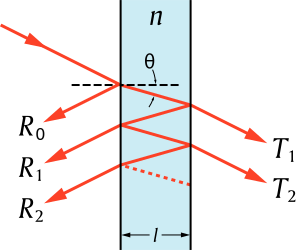
\includegraphics[width=0.95\linewidth]{Images/EtalonDiagram}
					\caption{Cross-section of the Fabry-Perot etalon. Light entering the etalon undergoes multiple internal reflections before being reflected or transmitted externally.}
					\label{fig:Fabry-Perot}
				\end{figure}
				
				In the diagram shown in figure \ref{fig:Fabry-Perot}, the difference in path length between light rays 1 and 2 is given by
				\begin{equation}
					\Delta l = DA + AB - CB 
				\end{equation}
				\begin{equation}
					= \frac{d}{Cos\theta} + \frac{d}{Cos\theta} - 2d(Sin\theta)Tan\theta
				\end{equation}
				\begin{equation}
					= \frac{2d}{Cos\theta} - \frac{2dSin^2\theta}{Cos\theta} =2dCos\theta
				\end{equation}
				Where $d$ is the gap distance of the etalon, approximately 1.995 mm.
				
				We can expand $Cos\theta$ in a Taylor series and only keep the first two terms because $\theta$ is very small
				\begin{equation}
					2dCos\theta = 2d\left(1-\frac{\theta^2}{2}\right)
				\end{equation}
				
				Thus, the total path length difference of the two rays is
				\begin{equation}
					\Delta l = 2d\left(1-\frac{\theta^2}{2}\right)
					\label{eq:EtalonPathLengthDiff}
				\end{equation}
				
				The two rays will be in phase and produce an interference maximum if and only if
				\begin{equation}
					\Delta l = (n+k)\lambda, k = 0, 1, 2, 3, ...
				\end{equation}
				
				Thus equation (\ref{eq:EtalonPathLengthDiff}) gives us
				\begin{equation}
					2d\left(1-\frac{\theta_k^2}{2}\right) = (n_k)\lambda, k = 0, 1, 2, 3,...
				\end{equation}
				where $\theta_k$ is the angle to the $k-th$ interference ring.
				See figure \ref{fig:B=0Pattern} for an example of the interference pattern seen through the Fabry-Perot etalon.
				
				Given a camera focal length f as shown in figre \ref{fig:CameraGeometry}, we can approximate the angle $\theta_k$ to be $\theta_k = R_k/f$, giving us
				\begin{equation}
					2d\left(1 - \frac{R_k^2}{2f^2}\right) = (n-k)\lambda, k=1,2,3,...
					\label{eq:Rk}
				\end{equation}
				
				We can get around not knowing the camera focal length using a measurement of the $B=0$ interference rings.
				For the $k=0$ ring, we have
				\begin{equation}
					2d\left(1-\frac{R_0^2}{2f^2}\right) = n\lambda
					\label{eq:R0}
				\end{equation}
				
				Subtracting equation (\ref{eq:Rk}) from (\ref{eq:R0}), we arrive at
				\begin{equation}
					\frac{d}{f^2}\lambda = \frac{k}{R_k^2 - R_0^2} = C_0
					\label{eq:ConstantEq}
				\end{equation}
				
				Thus by measuring the $R$ values for the interference rings with $B=0$, we can determine $C_0$.
				
				\begin{figure}
					\centering
					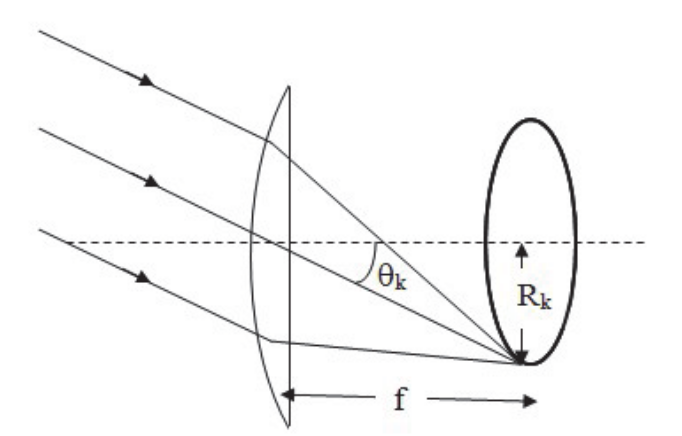
\includegraphics[width=0.95\linewidth]{Images/CameraGeometry}
					\caption{The camera lens geometry. Figure 4 from \cite{brolight_technology_co._ltd._zeeman_????}}
					\label{fig:CameraGeometry}
				\end{figure}

			\subsubsection{Final Derivation of the Bohr Magneton Equation}
				
				With equation (\ref{eq:Rk}), we have a general expression relating the interference rings' radial measurements to their wavelengths.
				Thus, we could measure the inner and outer rings of the hyperfine structure and take the difference to get the difference in wavelength between them.
				We thus arrive at
				\begin{equation}
					\left(\frac{d}{f^2}\right)\left(R_{k+}^2 - R_{k-}^2\right) = (n-k)(\lambda_- - \lambda_+)
				\end{equation}
				where $R_{k+}$ is the outer ring radius, $R_{k-}$ is the inner ring radius, $\lambda_+$ is the outer ring's wavelength, and $\lambda_-$ the inner ring's wavelength.
				
				Using equation (\ref{eq:WavelengthEq}) and the approximation $(n-k)\lambda = n\lambda = 2d$ and solving for the Bohr magneton, we have
				\begin{equation}
					\mu_B = \left( \frac{C_0 hc}{2dB} \right) \left( R_{k+}^2 - R_{k-}^2 \right)
					\label{eq:BohrEquation}
				\end{equation}
				
				We will use this equation in Section \ref{subsec:BohrCalc} to calculate an experimental value for the Bohr magneton.
		

		
\section{Methods and Procedures}
	The Pasco Scientific Model SE-9654 Zeeman Effect Experiment was used to make all observations.
	The experiment consisted of two large solenoids oriented along the same axis with an air gap between them in which a mercury lamp was placed.
	An optical rail was used to align a polarizing filter, a collimating lens, an interference filter, a Fabry-Perot interferometer, and a CMOS camera.
	The basic experimental technique consisted of imaging the interference pattern of the 546.1 nm mercury spectral line with the CMOS camera through the polarizer and Fabry-Perot interferometer.
	Figures \ref{fig:ContextView} and \ref{fig:SolenoidDetail} show the optics bench setup, including the solenoid electromagnet.
	
	\begin{figure*}
		\centering
		\begin{subfigure}{0.5\textwidth}
			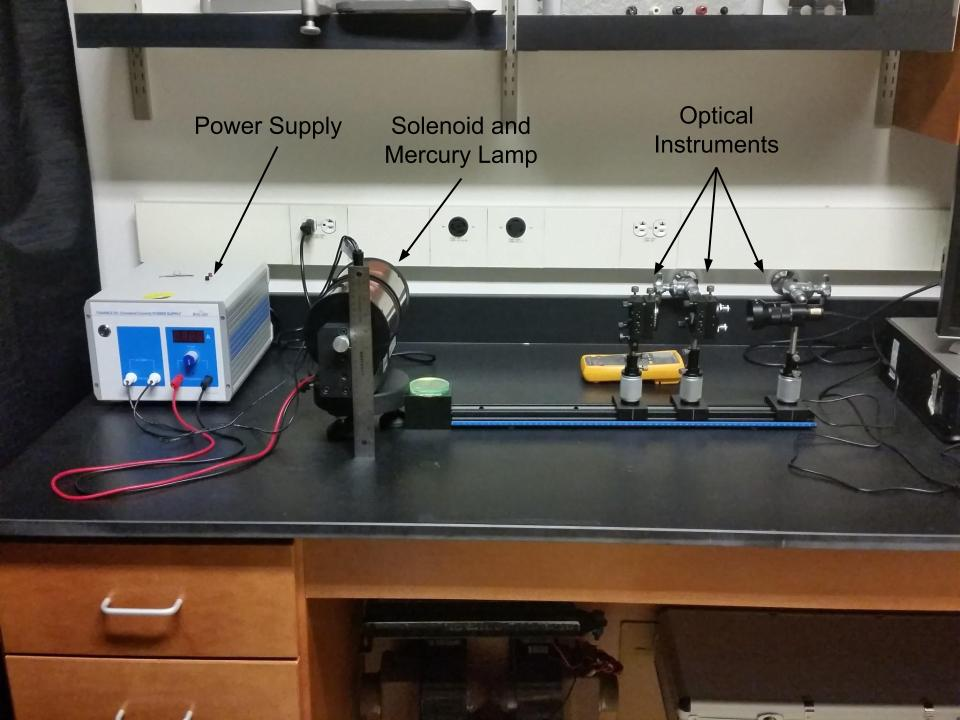
\includegraphics[width = 0.98\textwidth]{Images/ExperimentOverview.jpg}
			\caption{}
			\label{subfig:Overview}
			
		\end{subfigure}%
		\begin{subfigure}{0.5\textwidth}
				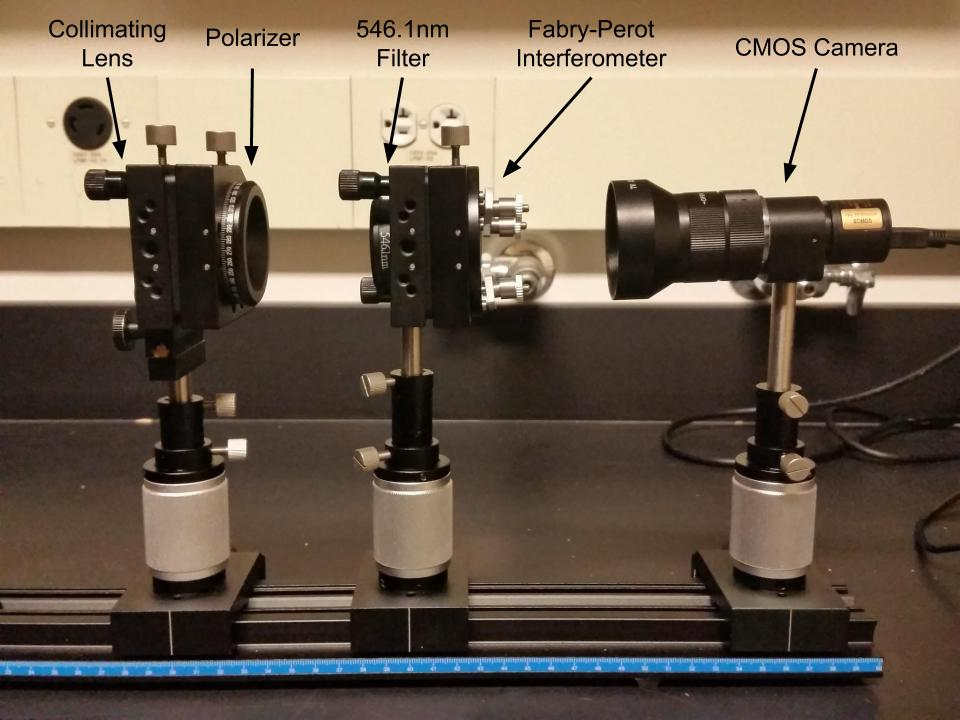
\includegraphics[width = 0.98\textwidth]{Images/OpticsRail.jpg}
				\caption{}
				\label{subfig:OpticsRail}
				
		\end{subfigure}%
		\caption{Overview of the Experiment configuration. Figure \ref{subfig:Overview} shows the entire apparatus with the variable power supply for the solenoid and mercury lamp, the solenoid, the mercury lamp (hidden by the solenoid), the optical track, and the optical instruments. Figure \ref{subfig:OpticsRail} shows the optical instruments in detail.}
		\label{fig:ContextView}
	\end{figure*}
	
	\begin{figure*}
		\centering
		\begin{subfigure}{0.5\textwidth}
			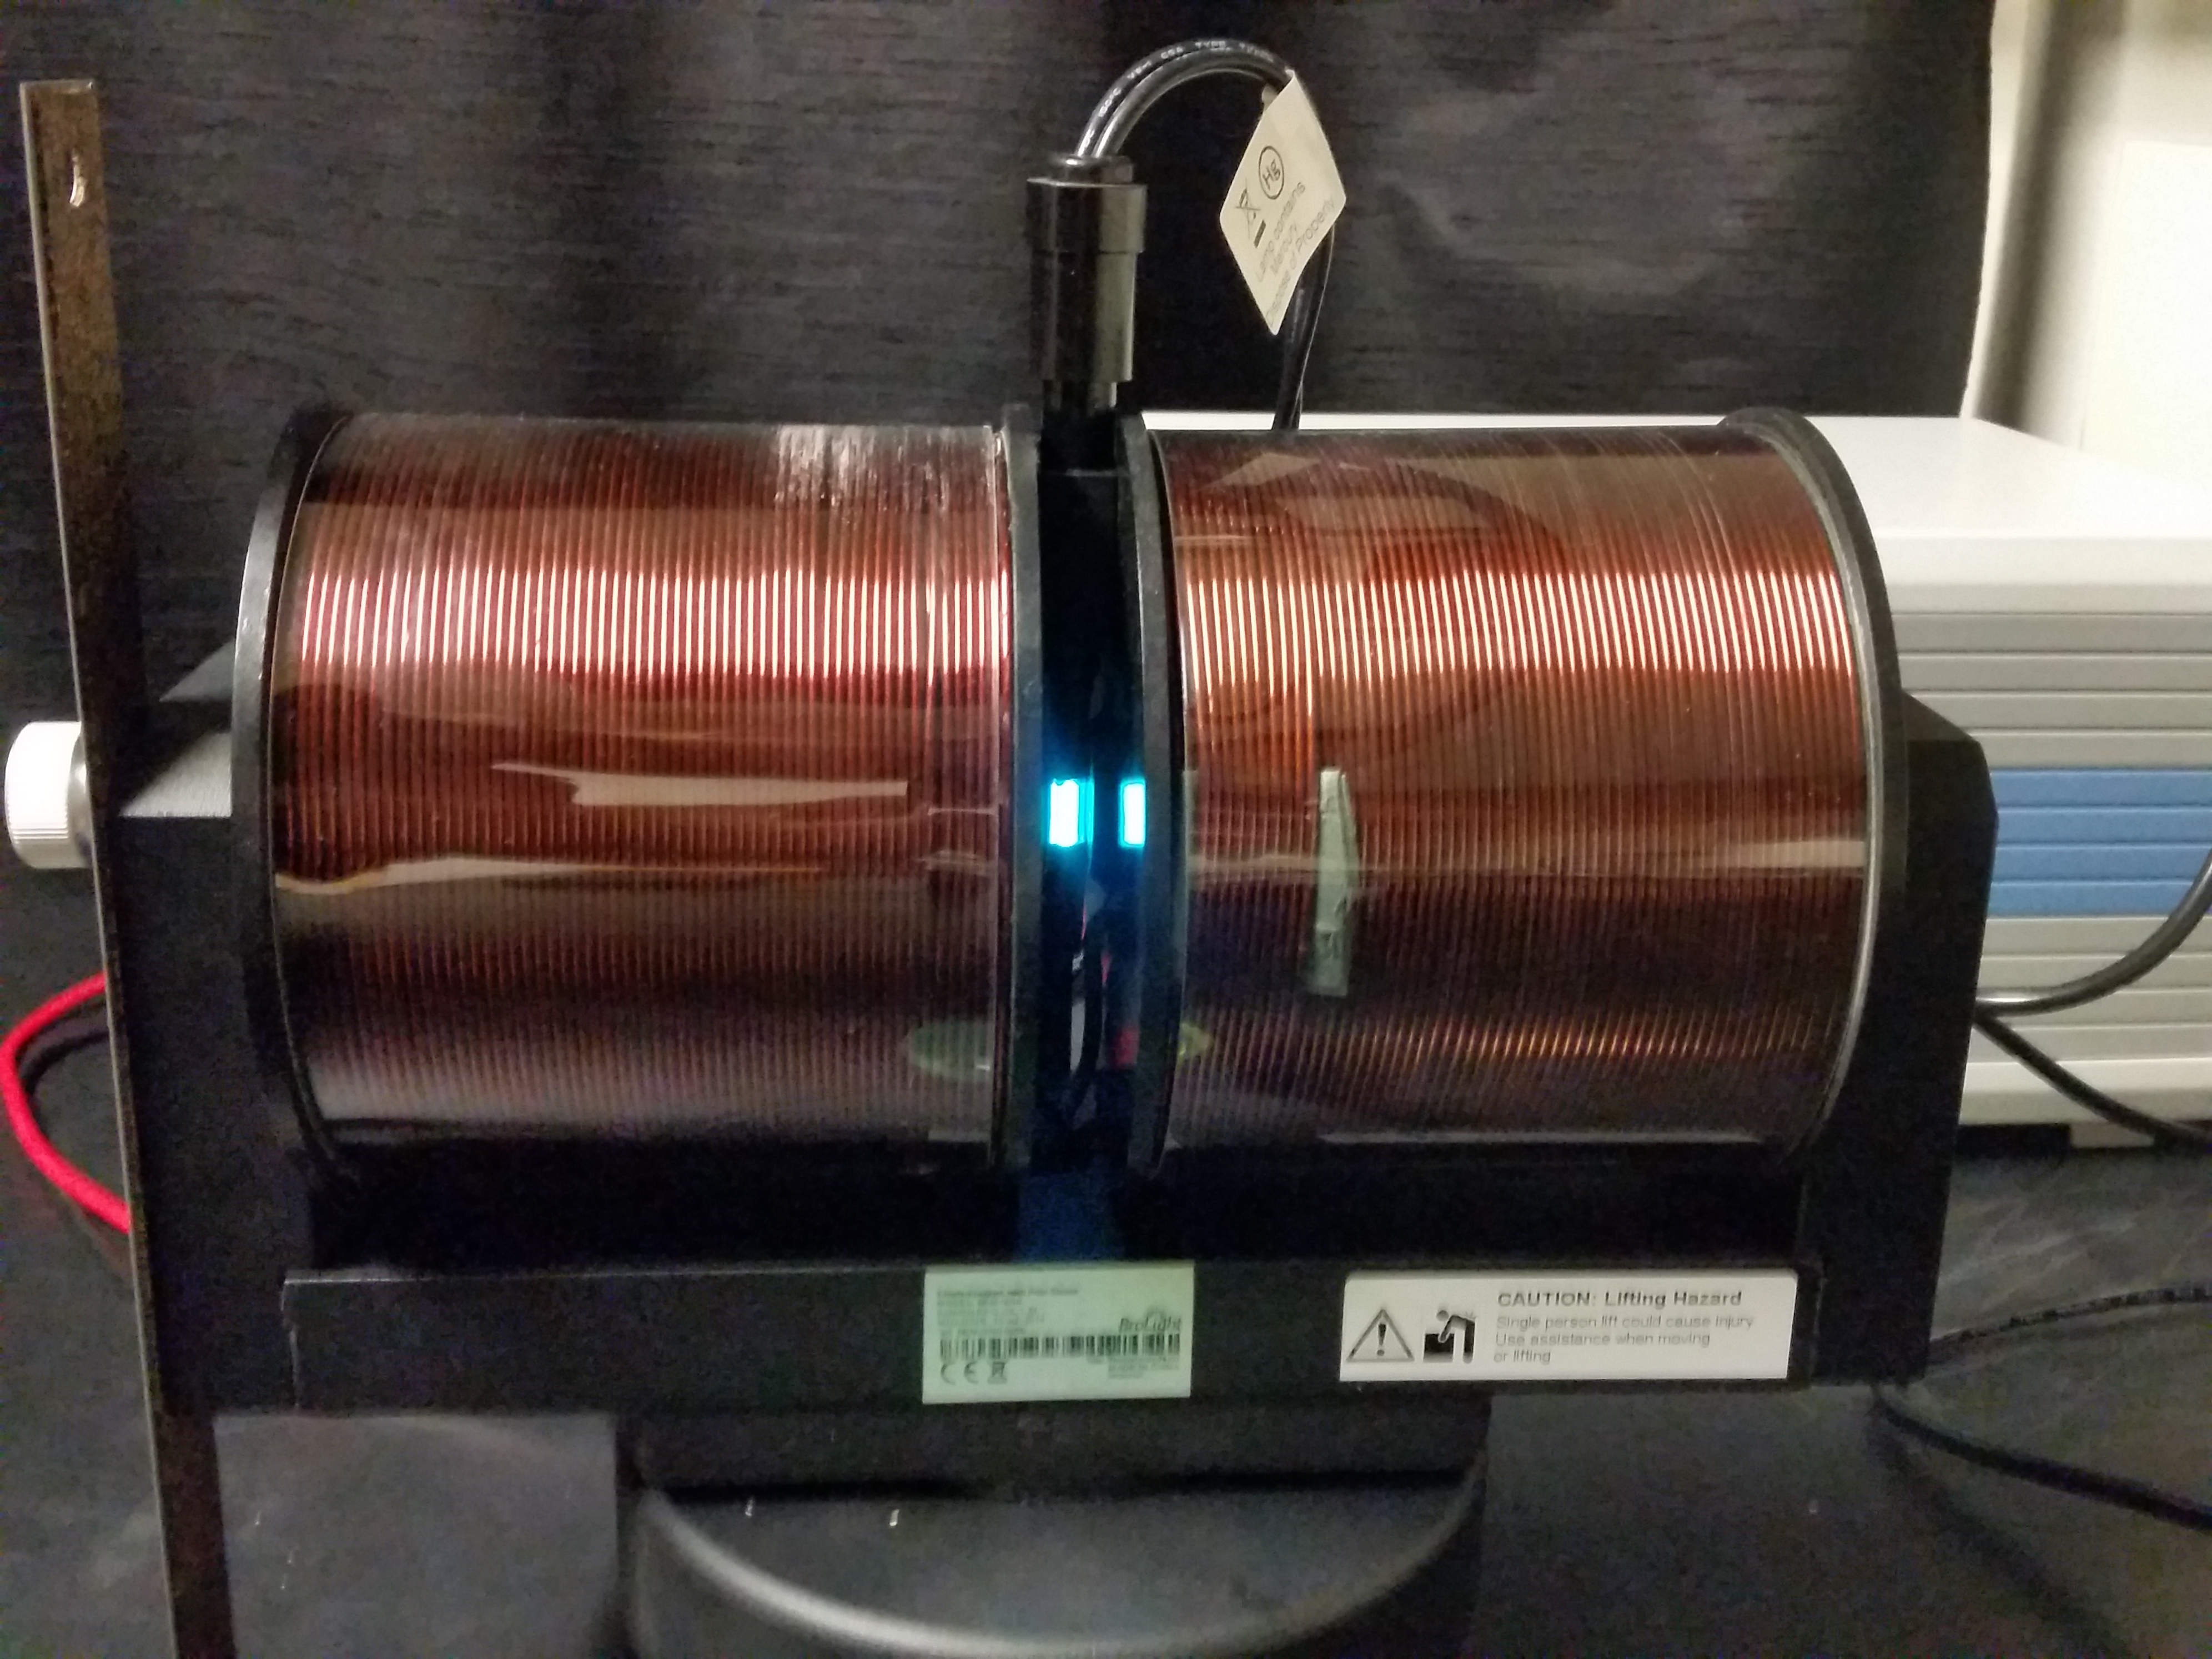
\includegraphics[width = 0.98\textwidth]{Images/PerpendicularView.jpg}
			\caption{}
			\label{subfig:PerpView}
		\end{subfigure}%
		\begin{subfigure}{0.5\textwidth}
			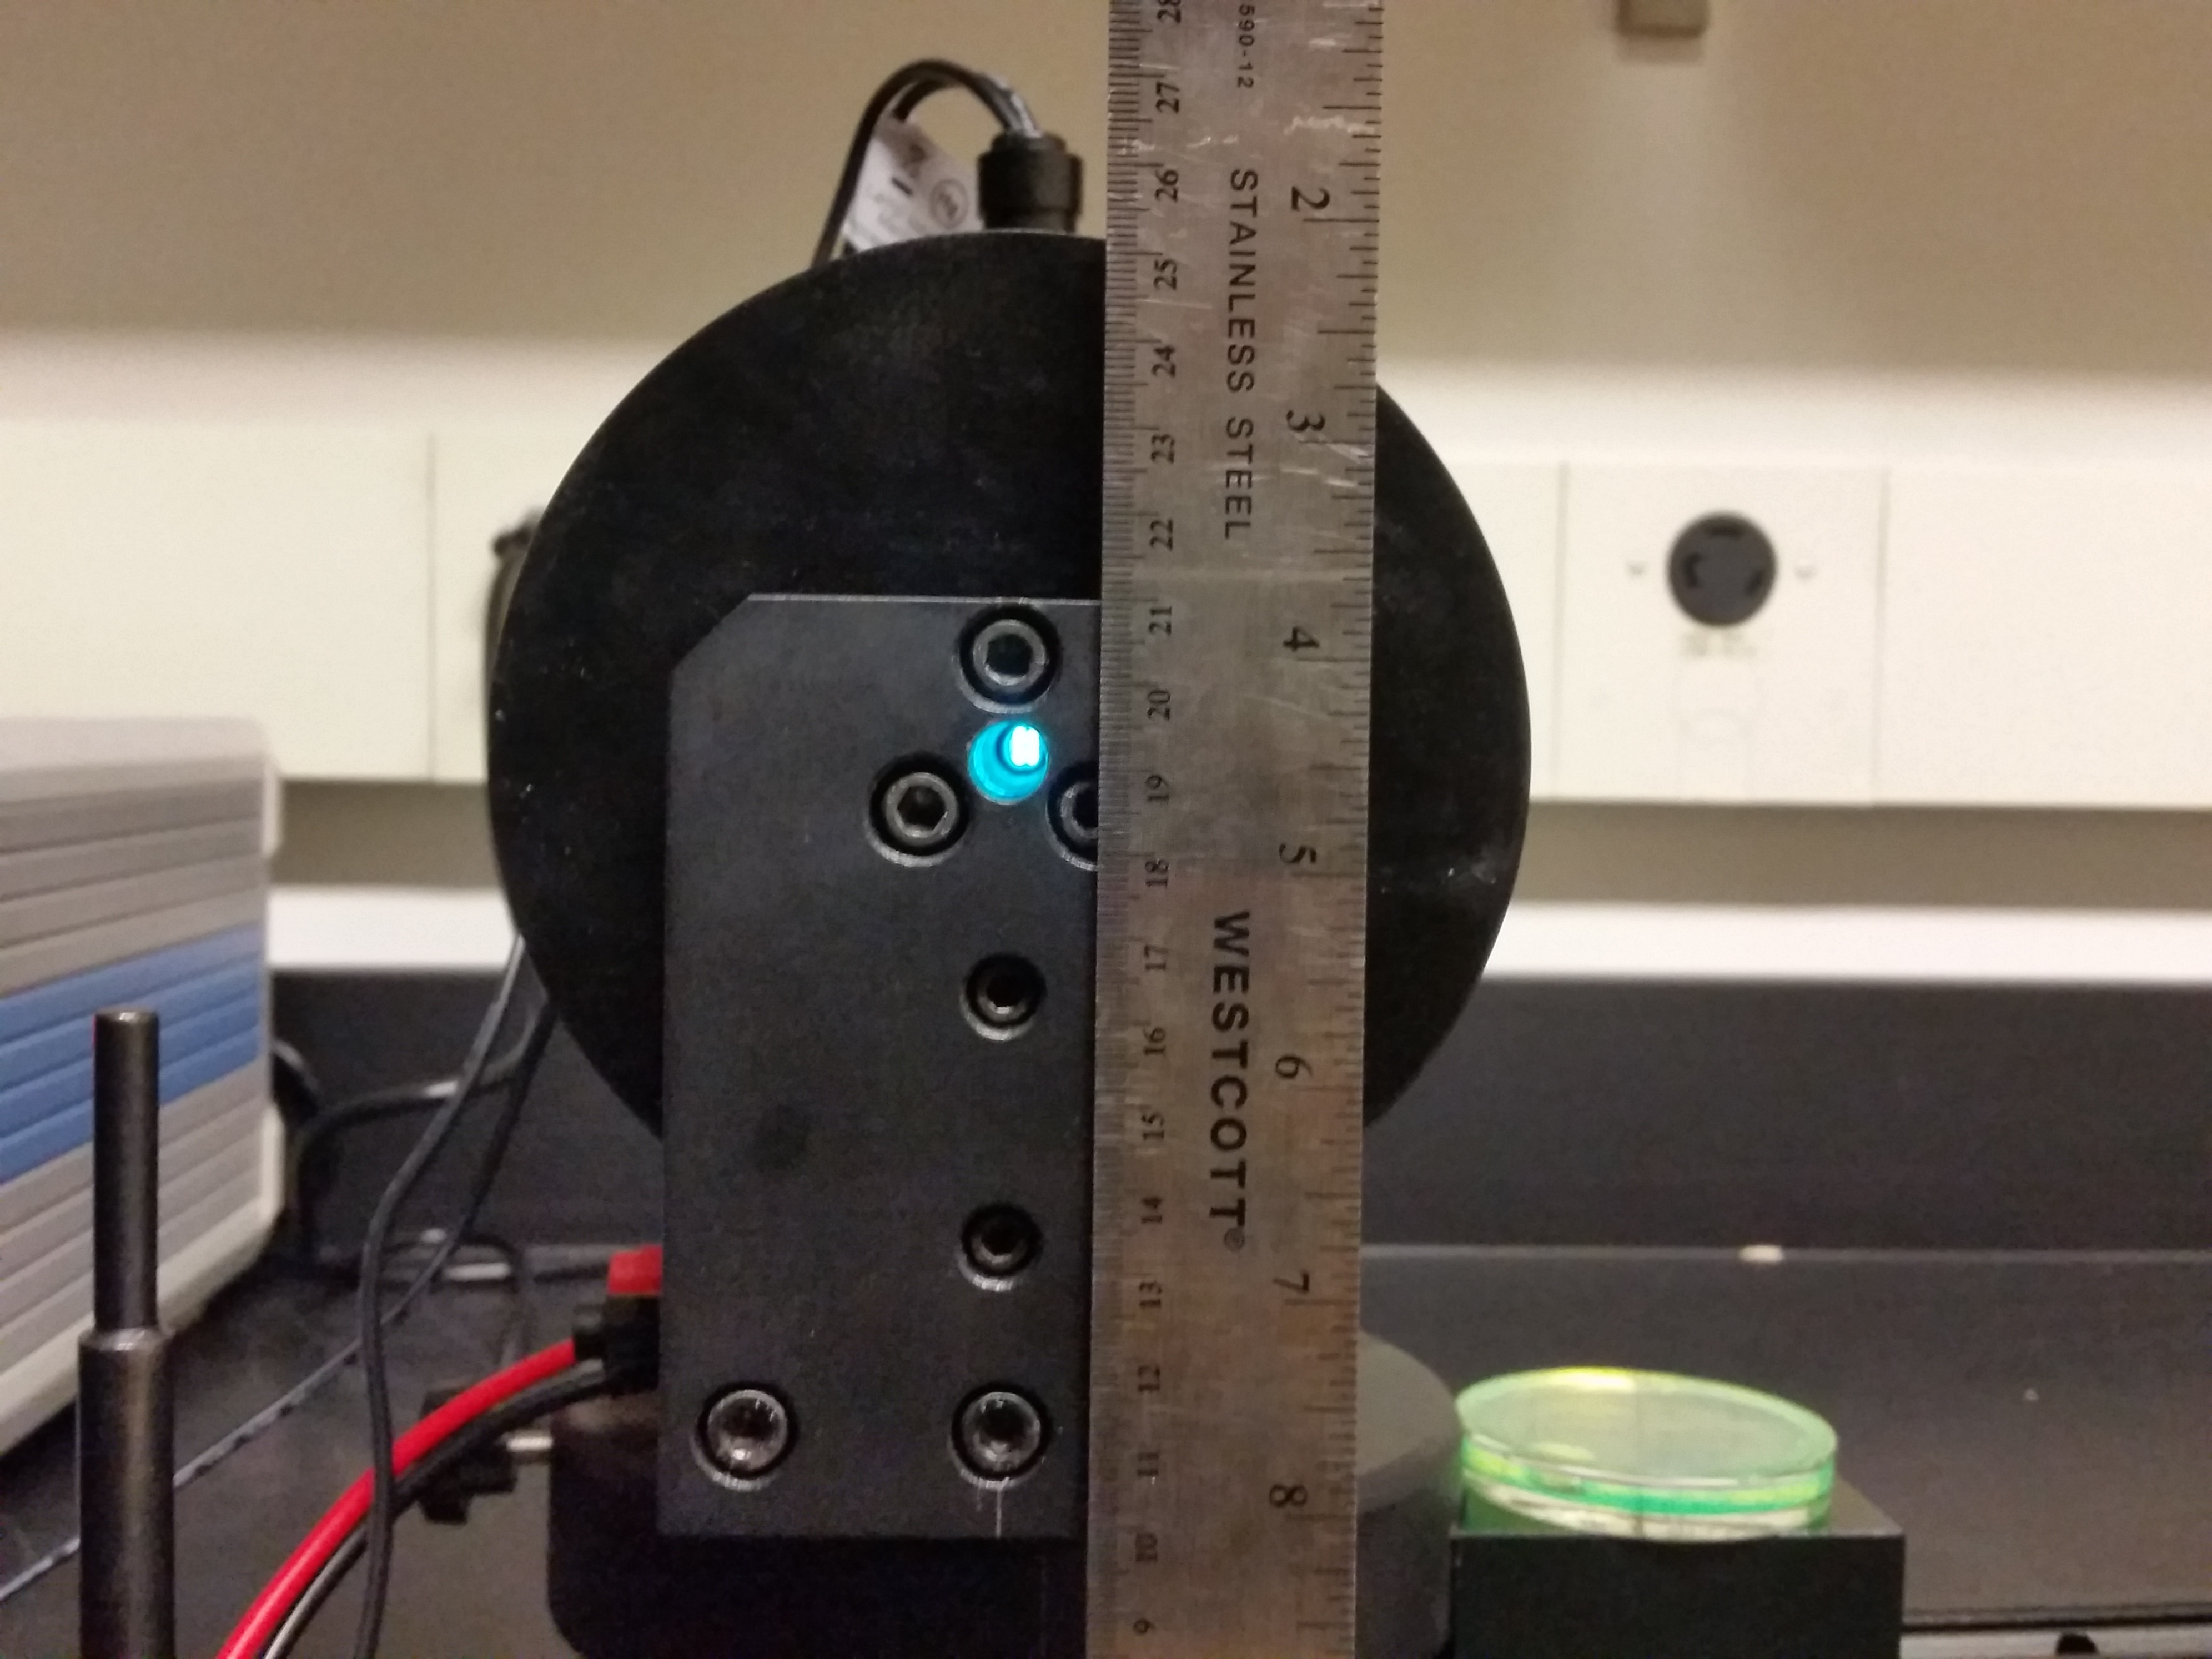
\includegraphics[width = 0.98\textwidth]{Images/AxialView.jpg}
			\caption{}
			\label{subfig:AxialView}
		\end{subfigure}%
		\caption{Detail view of the solenoid with the mercury lamp source. Figure \ref{subfig:PerpView} shows the configuration with the magnetic field lines perpendicular to the light source. Figure \ref{subfig:AxialView} shows the axial field configuration looking down the sight-hole of the solenoid to the mercury lamp.}
		\label{fig:SolenoidDetail}
	\end{figure*}
	
	To study the Zeeman effect, observations of a mercury lamp were made first with no magnetic field and $90\deg$ polarization, then with an approximately $1T$ magnetic field.
	Observations with a magnetic field included:
	\begin{itemize}
		\item No polarization
		\item Field-parallel polarization
		\item Field-perpendicular polarization 
		\item Axial B-field
	\end{itemize}
	
	Figure \ref{fig:FieldConfig} shows the perpendicular and axial configurations of the magnetic field used for the observations.
	
	The observations and results of each of these field configurations will be presented and discussed in Section \ref{sec:DataAndResults}.
	
	\begin{figure*}
		\centering
		\begin{subfigure}{0.5\textwidth}
			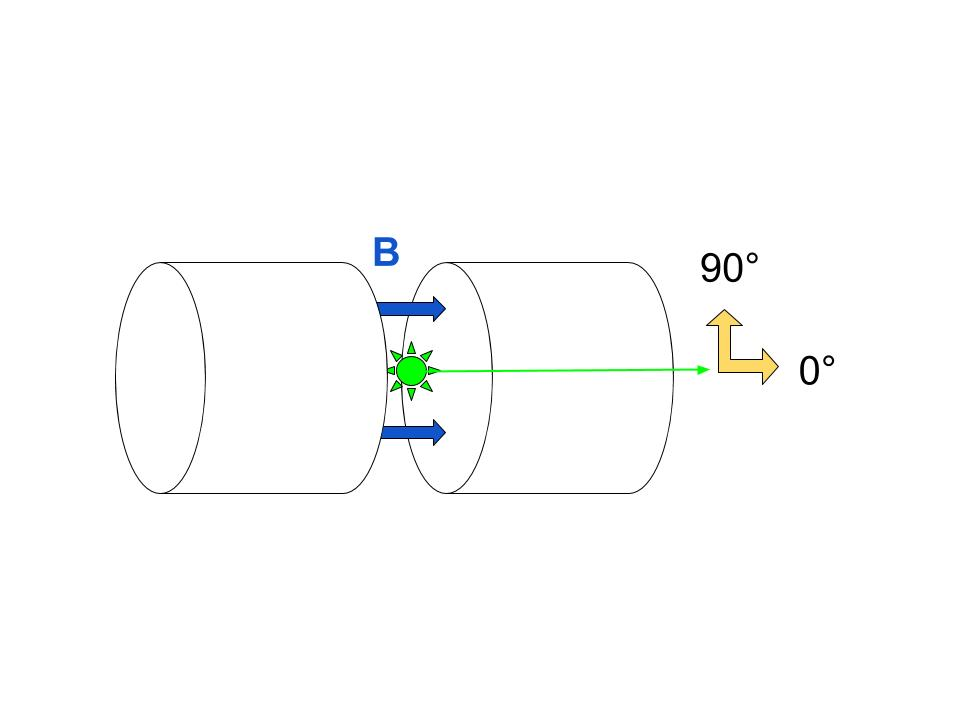
\includegraphics[width = 1.0\textwidth]{Images/FieldConfigA.jpg}
			\caption{Perpendicular field configuration.}
			\label{subfig:PerpFieldConfig}
		\end{subfigure}%
		\begin{subfigure}{0.5\textwidth}
			\centering
			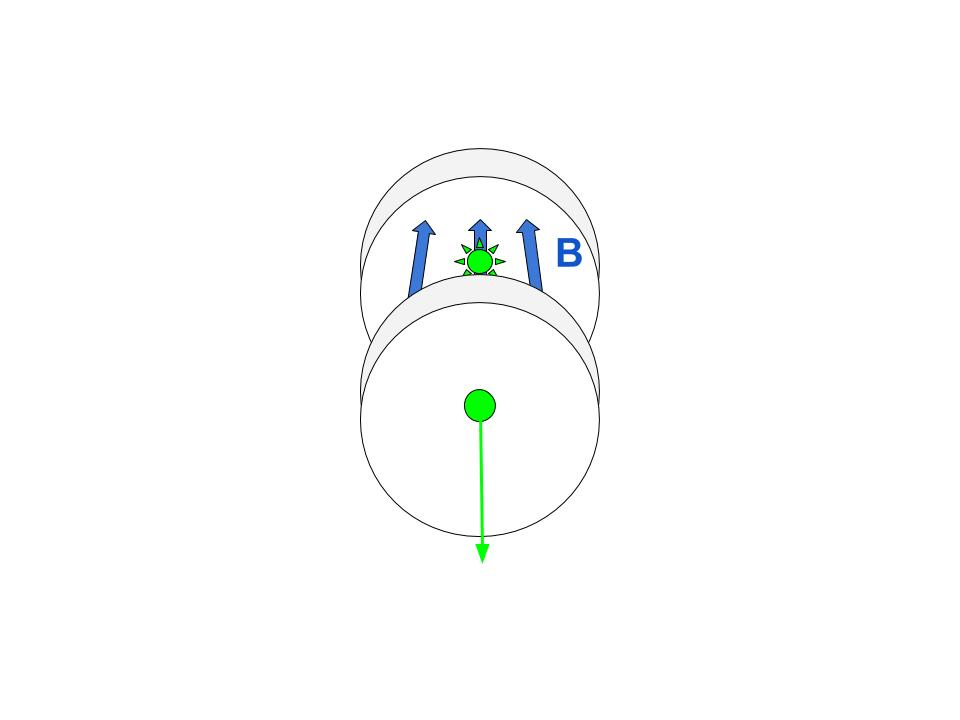
\includegraphics[width=1.0\textwidth]{Images/FieldConfigB.jpg}
			\caption{Axial field configuration.}
			\label{subfig:AxialFieldConfig}
		\end{subfigure}%
		\caption{The two magnetic field configurations observed. In (\ref{subfig:PerpFieldConfig}), the magnetic field is oriented perpendicularly to the path of the observed light from the mercury lamp. $90\degree$ polarization is defined to be perpendicular to the field lines, while $0\degree$ polarization is parallel to the field lines. In configuration (\ref{subfig:AxialFieldConfig}), light from the lamp travels along the magnetic field lines down the center of one of the solenoids through a sight hole.}
		\label{fig:FieldConfig}
	\end{figure*}
	
\section{Data and Results} \label{sec:DataAndResults}
	 
	 With no applied magnetic field, the 546.1nm mercury spectral line as viewed through the Fabry-Perot interferometer produces the interference pattern as shown in Figure \ref{fig:B=0Pattern}.
	 The $B=0$ interference pattern shows discrete rings, with the innermost ring denoted as the $k=0$ ring, the next innermost ring the $k=1$ ring, and so on.
	 
	 \begin{figure*}
	 	\centering
	 	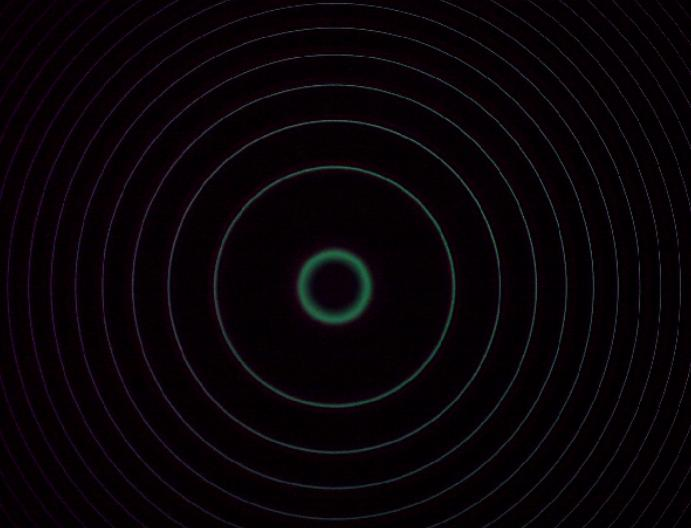
\includegraphics[width=0.65\linewidth]{Images/B=0Pattern}
	 	\caption{Interference pattern of the 546.1nm mercury line with no applied magnetic field. The interference lines are singular.}
	 	\label{fig:B=0Pattern}
	 \end{figure*}
	 
	 Table \ref{tab:B0Data} shows the measured radii of the interference rings for the $k=1$ through $k=4$ rings.
	 The $k=0$ ring was not used in subsequent observations and calculations because it was not resolved enough to be measurable.
	 
	 The ``bullseye'' $B=0$ pattern will be the standard interference pattern we will compare all subsequent patterns on.
	 
	\subsection{Observations perpendicular to the Magnetic Field}
		The first observations were made such that the mercury lamp was viewed perpendicularly to the magnetic field, as is shown in Figure \ref{subfig:PerpFieldConfig}.
		
		When viewed without a polarizer, the interference pattern appears as in Figure \ref{fig:Run2_NoPolarizer_detail}.
		All nine of the transition spectra, corresponding to all nine possible unique $\Delta M_j$ transition values, can be seen.
		
		\begin{figure*}
			\centering
			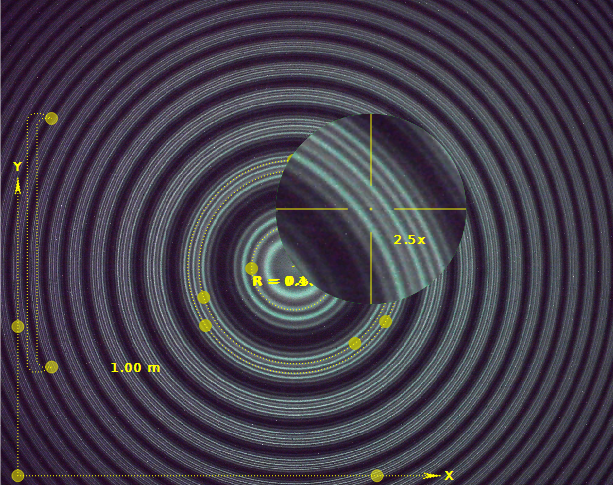
\includegraphics[width=0.6\linewidth]{Images/Run2_NoPolarizer_detail}
			\caption{Mercury spectra in the presence of a magnetic field viewed without a polarizer. All spectra from all nine unique $\Delta M_j$ transitions can be seen.}
			\label{fig:Run2_NoPolarizer_detail}
		\end{figure*}

		From the theory discussed in section \ref{sec:Theory}, different values of $\Delta M_j$ in the mercury transition will produce different polarizations of the emitted light.
		Thus, we can use polarization to identify particular hyperfine lines which correspond to certain values of $\Delta M_j$.
		
		\subsubsection{$\mathbf{\Delta M_j = 0}$ Transition spectra}
			With a $1T$ magnetic field and the polarizer set parallel to the field lines, we observed the mercury spectra with polarization parallel to the applied magnetic field. A distinct triple ring structure can be seen Figure \ref{fig:Triplet90deg} in which each interference ring consists of a bright central ring surrounded by two fainter rings. 
			This is what has been historically termed the ``Normal" Zeeman effect.
			
			\begin{figure*}
				\centering
				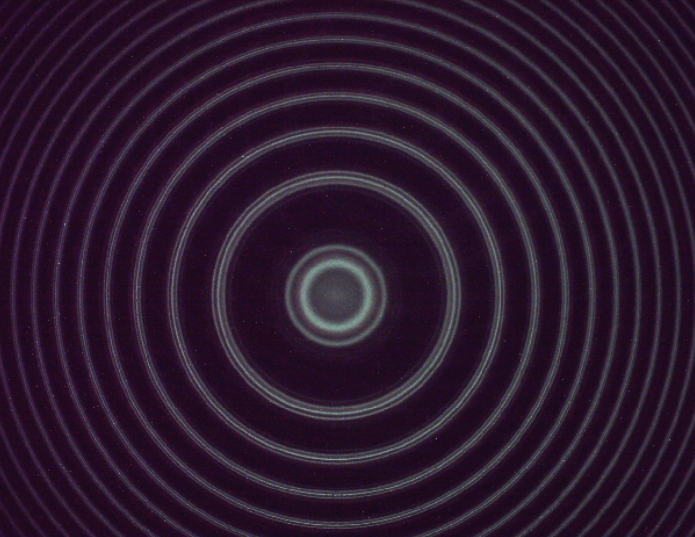
\includegraphics[width=0.6\linewidth]{Images/Run1_ParallelPolarizer}
				\caption{The ``Normal" Zeeman effect. Mercury interference pattern viewed perpendicular to the magnetic field lines through a polarizer oriented parallel to the field. The interference rings correspond to photons produced by $\Delta M_j = 0$ transitions polarized parallel to the magnetic field lines.}
				\label{fig:Triplet90deg}
			\end{figure*}
			
			Using PASCO Software, The radii of the inner and outer rings of the $k=1$ through $k=4$ interference rings were measured.
			These radii are given in Table \ref{tab:RadiusMeasurements} and will be used to calculate the value of the Bohr magneton in Section \ref{subsec:BohrMagneton}.
			\begin{table*}[]
				\centering
				\begin{tabular}{l|lll}
					k = 1 & & & \\
					Measurements & $R+$ (m) & $R-$ (m)  & $\Delta$R (m) \\ \hline
					1         & 0.4282 & 0.3893  & 0.0389 \\
					2         & 0.4278 & 0.3896  & 0.0382 \\
					3         & 0.4275 & 0.3887  & 0.0388 \\
					Mean      & $0.4278\pm0.4\times10^{-3}$       & $0.3892\pm0.5\times10^{-3}$        & $0.039\pm0.4\times10^{-3}$ \\ \hline
					k = 2 & & & \\
					Measurements & $R+$ (m) & $R-$ (m)  & $\Delta$R (m) \\ \hline
					1           & 0.5819 & 0.5539 & 0.0280 \\
					2           & 0.5815 & 0.5536 & 0.0279 \\
					3           & 0.5818 & 0.5536 & 0.0282 \\
					Mean        & $0.5817\pm0.2\times10^{-3}$ & $0.5537\pm0.2\times10^{-3}$ & $0.0280\pm0.2\times10^{-3}$ \\ \hline
					k = 3 & & & \\
					Measurements & $R+$ (m) & $R-$ (m)  & $\Delta$R (m) \\ \hline
					1    & 0.7035 & 0.679  & 0.0245 \\
					2    & 0.7033 & 0.6798 & 0.0235 \\
					3    & 0.7025 & 0.6805 & 0.0220 \\
					Mean & $0.7031\pm0.5\times10^{-3}$ & $0.6798\pm0.8\times10^{-3}$ & $0.0233\pm0.001$ \\ \hline
					k = 4 & & & \\
					Measurements & $R+$ (m) & $R-$ (m)  & $\Delta$R (m) \\ \hline
					1    & 0.8058 & 0.7861 & 0.02  \\
					2    & 0.8057 & 0.7865 & 0.02  \\
					3    & 0.8059 & 0.7857 & 0.02  \\
					Mean & $0.8058\pm0.1\times10^{-3}$ & $0.7861\pm0.4\times10^{-3}$ & $0.020\pm0.001$
				\end{tabular}
				
				
				\caption{Radius measurements of the hyperfine structure of the k=1 through k=4 interference rings with a 1T magnetic field and $\mathbf{90\degree}$ polarization.}
				\label{tab:RadiusMeasurements}
			\end{table*}
			
		\subsubsection{$\mathbf{\Delta M_j = \pm1}$ Transition Spectra}
			By orienting the polarizer perpendicular to the magnetic field lines, we were able to observe the spectra due to the circularly-polarized $\Delta M_j = \pm1$ transitions.
			The result is shown in figure \ref{fig:Run2_0Deg}, in which it can be seen that each interference ring is now missing the $\Delta M_j=0$ rings which have been filtered by the polarizer, while the outer rings due to the $\Delta M_j = \pm1$ transitions are visible.
			
		\begin{figure*}
			\centering
			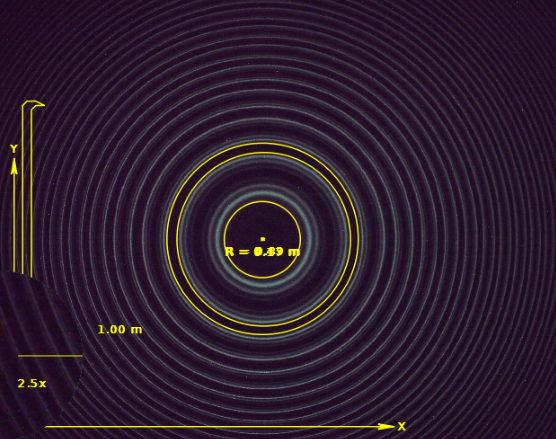
\includegraphics[width=0.55\linewidth]{Images/Run2_PerpendicularPolarizer}
			\caption{Interference pattern viewed through a polarizer oriented perpendicular to the magnetic field lines. The $\Delta M_j = 0$ transition spectra polarized parallel to the magnetic field cannot be seen, leaving a large gap between the circularly-polarized $\Delta M_j = \pm1$ transition spectra.}
			\label{fig:Run2_0Deg}
		\end{figure*}

		
	\subsection{Spectra Along an Axial Magnetic Field}
		Our next observation was axial with the magnetic field, as shown in figures \ref{subfig:AxialFieldConfig} and \ref{subfig:AxialView}.
		The result is shown in figure \ref{fig:Run3_AxialField}.
		Regardless of whether a polarizer was used or not, and indeed regardless of the orientation of the polarizer, the pattern did not change.
		This agrees with the theory, as the linearly-polarized $\Delta M_j = 0$ transitions cannot propagate axially, as their field vectors $\mathbf{E}$ and $\mathbf{B}$ must be mutually perpendicular with their propagation direction.
		
		The circularly-polarized $\Delta M_j = \pm1$ transitions can be seen, however, as they are polarized circularly about the magnetic field lines.
		
		\begin{figure*}
			\centering
			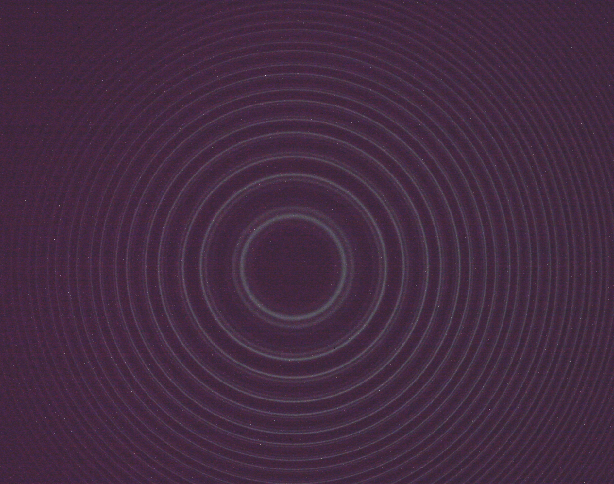
\includegraphics[width=0.55\linewidth]{Images/Run3_AxialField}
			\caption{Interference pattern viewed axially along the magnetic field through the sight-hole in the electromagnet as shown in Figure \ref{subfig:AxialFieldConfig}. Only the circularly-polarized $\Delta M_j = \pm1$ transition spectra can be seen since photons from the $\Delta M_j = 0$ transition spectra cannot propagate in this direction because their $\mathbf{E}$ and $\mathbf{B}$ field vectors must be perpendicular to their propagation direction.}
			\label{fig:Run3_AxialField}
		\end{figure*}

	\subsection{Measurement of the Bohr Magneton} \label{subsec:BohrMagneton}
		Using the measurements of the split interference rings from the observation of the ``Normal" Zeeman effect with the $\Delta M_j = 0$ transition spectra, we were able to establish a value for the Bohr magneton.
		The inner and outer radius of each interference triplet was measured using PASCO software and is tabulated in Table \ref{tab:RadiusMeasurements}.
		
		To calculate the magnitude of the Bohr magneton, we use the theory from Section \ref{subsec:BohrCalc}.
		First, we must calculate the constant $C_0$ in equation (\ref{eq:ConstantEq}).
		This is accomplished using the un-split interference ring radii from the $B=0$ case.
		These measurements are given in Table \ref{tab:B0Data}.
		
		\begin{table}[h]
			\centering
			\begin{tabular}{l|l}
				k & Radius (m) \\ \hline
				4 & 0.7956 $\pm$ $0.1\times10^{-3}$    \\
				3 & 0.6911 $\pm$ $0.2\times10^{-3}$    \\
				2 & 0.5678 $\pm$ $0.1\times10^{-3}$    \\
				1 & 0.4096 $\pm$ $0.1\times10^{-3}$   
			\end{tabular}
			\caption{Interference ring radii of the mercury 546.1 nm spectra with no magnetic field.}
			\label{tab:B0Data}
		\end{table}
		
		Using equation (\ref{eq:ConstantEq}), the value of $C_0$ for each interference ring $k=1$ through $k=4$ was calculated.
		The average of these values was then taken as the best value for $C_0$.
		Table \ref{tab:C0} lists the calculated values for each interference ring, as well as the overall mean and standard deviation.
		
		\begin{table}[]
			\centering
			\begin{tabular}{l|l}
				k & $C_0$ $(m^{-2})$ \\ \hline
				4 & 6.4523 \\
				3 & 6.4575 \\
				2 & 6.4633 \\
				1 & 6.4598 \\ \hline
				Mean & $6.458\pm0.005$
			\end{tabular}
			\caption{Measured values of the constant $C_0$ from the $B=0$ interference rings.}
			\label{tab:C0}
		\end{table}
		
		With a precise measured value for $C_0$, values for the Bohr magneton can then be calculated with equation (\ref{eq:BohrEquation}).
		The difference between inner and outer radii for each interference ring in the $B\neq 0$, parallel-field polarization case, which is related to the magnitude of the change in wavelength between the $\Delta M_j = \pm1$ transitions, is used to calculate the Bohr magneton.
		These values for $R_{k+}$ and $R_{k-}$ are given in Table \ref{tab:RadiusMeasurements}.
		
		The remaining constants in equation (\ref{eq:BohrEquation}) are Planck's constant, $h = 6.63\times10^{-34}$, the speed of light, $c = 2.99\times10^8 m/s$, the gap distance of the Fabry-Perot etalon, $d = 1.995\times10^{-3} m$, and the magnitude of the magnetic field at $5 A$, $B = 1.105 T$.
		
		The calculated values for the Bohr magneton for each interference ring as well as the mean and standard deviation are given in Table \ref{tab:BohrCalcs}.
		
		\begin{table}[]
			\centering
			\begin{tabular}{l|l}
				$k$  & $\mu_B \ (J\cdot T^{-1})$ \\ \hline
				1    & $9.16\times10^{-24}$   \\
				2    & $9.24\times10^{-24}$   \\
				3    & $9.36\times10^{-24}$   \\
				4    & $9.10\times10^{-24}$   \\ \hline
				Mean & $9.22\times10^{-24}\pm0.06\times10^{-24}$  
			\end{tabular}
			\caption{Calculated values of the Bohr magneton $\mu_B$ for each interference ring, and the mean calculated value for all interference rings.}
			\label{tab:BohrCalcs}
		\end{table}
		
		Our calculated best value for the magnitude of the Bohr magneton is thus 
		\begin{equation}
			\mu_B = 9.22\times10^{-24}\pm 0.06\times10^{-24} J\cdot T^{-1}
		\end{equation}
		
		For comparison, the SI value of the Bohr magneton is $9.274\times10^{-24} J\cdot T^{-1}$\cite{_codata_????}, which is within our margin of measured random error.
		Additionally, our measured value agrees with the accepted SI value to within 0.63\%.
		

\section{Conclusion} \label{sec:Conclusion}
	We observed the Zeeman  effect and verified its effect on the 546.1 nm mercury spectral line in the presence of a $\approx1T$ magnetic field.
	We verified that the hyperfine structure was produced by transitions of various changes of the quantum number $\Delta M_j$ which are constrained by the quantum selection rules.
	Using a polarizer, we showed that the different hyperfine spectra have either parallel or circular polarization along the magnetic field lines.
	We were able to separately observe light polarized parallel to the magnetic field lines created in $\Delta M_j = 0$ transitions, as well as axially circular-polarized light created in $\Delta M_j = \pm1$ transitions.
	Finally, we arrived at a measured value for the Bohr magneton of $\mu_B = 9.22\times10^{-24}\pm 0.06\times10^{-24} J\cdot T^{-1}$, which is consistent with the modern accepted SI value to within 0.63\%.
\bibliographystyle{ieeetr}
\bibliography{ZeemanPaper}

\end{document}
